%%%%%%%%%%%%%%%%%%%%%%%%%%%%%%%%%%%%%%%
% Important notes:
% This template needs to be compiled with XeLaTeX.
%
%%%%%%%%%%%%%%%%%%%%%%%%%%%%%%%%%%%%%%

\documentclass[letterpaper]{style} % Use US Letter paper, change to a4paper for A4 
\usepackage{fontawesome}
\usepackage{graphicx}
\usepackage{hyperref}
\usepackage{array}
\usepackage{tikz}
\usetikzlibrary{shapes, calc, positioning, backgrounds, arrows,automata,mindmap}
\usepackage{adjustbox}
\usepackage{graphicx}
\def\ci#1{\textcircled{\resizebox{.5em}{!}{#1}}}

\begin{document}
%
\includegraphics[scale=0.065]{nitinFaceSmall.png}
\namesection{{nitin}}{bhushan\\
%\Large{data science | energy transition | %research}}
\large{data scientist | educator | consultant |}}
{
\href{mailto:bhushan.nitin@posteo.net}{\ci{\faEnvelope}} {\fontsize{8}{8}\selectfont \href{mailto:bhushan.nitin@posteo.net}{bhushan.nitin@posteo.net}}}
{
\ci{\faPhone}  {\fontsize{10}{10}\selectfont +31 644 024 293} 
}
{
\href{https://github.com/nbhushan}{\ci{\faGithub}} {\fontsize{9}{9}\selectfont \href{https://github.com/nbhushan}{nbhushan.github.io}}
}
{
\href{https://www.linkedin.com/in/bhushannitin/}{\ci{\faLinkedin}}
{\fontsize{9}{9}\selectfont  \href{https://www.linkedin.com/in/bhushannitin/}{nbhushan}}
}
\leavevmode \\
%\leavevmode \\
%%----------------------------------------------------------------------------------------
%	LEFT COLUMN
%----------------------------------------------------------------------------------------

\begin{minipage}[t]{0.33\textwidth} % The left column takes up 33% of the text width of the page

\section{Profile}
\tikz[remember picture] 
\node[circle,xshift=8cm, yshift=0cm, opacity=0.9] {

\includegraphics[width=2.8cm,height=3.0cm]{nbhushanCircle.png}
};

\emph{Curious about a data-driven world,\\ I spend my time connecting the dots\\ between engineering, data science \& AI,\\ and behavioural sciences.}

\vspace{8pt}

\section{Education} 
\runsubsection{PhD}
\descript{| data science}
\location{University of Groningen \\ Netherlands |  June 2020}
\vspace{\topsep} % Hacky fix for awkward extra vertical space
\vspace{1pt}
\begin{tightitemize}
\item topics: additive models, \\time series, graphical models,\\ causal inference
\item developed models to explore, understand, and predict the\\ human dimension of the\\ energy transition
\item advisors: \href{https://www.rug.nl/staff/e.m.steg/}{linda steg}, \href{https://www.rug.nl/staff/c.j.albers//}{casper albers} 
\end{tightitemize}
\vspace{7pt}

\runsubsection{MSc}
\descript{| Artificial Intelligence}
\location{Maastricht University\\Netherlands | 2013}
\begin{tightitemize}
\item foundations in \\probabilistic modelling 
\item relevant courses: data mining \& machine learning,text mining,\\and multi-agent systems 
\end{tightitemize}
\vspace{7pt}

\runsubsection{BE}
\descript{| Electrical engineering}
\location{MSRIT | Bangalore, India | 2009}
\begin{tightitemize}
\item foundations in energy systems 
\item relevant courses: \\applied mathematics,\\ control theory, \\energy technology,\\and power systems analysis
\end{tightitemize}
\vspace{8pt}

\sectionspace % Some whitespace after the section


%------------------------------------------------
% Coursework
%------------------------------------------------
\sectionspace % Some whitespace after the section
\end{minipage} % The end of the left column
\hfill
%
%----------------------------------------------------------------------------------------
%	RIGHT COLUMN
%----------------------------------------------------------------------------------------
%
\begin{minipage}[t]{0.66\textwidth} % The right column takes up 66% of the text width of the page

%------------------------------------------------
% Experience
%------------------------------------------------
\section{Experience}

\runsubsection{Breda University of Applied Sciences}
\descript{| data science educator}
\location{april 2021 - now | Breda, The Netherlands}
\vspace{\topsep}
\begin{tightitemize}
\item design and execute a project-based bachelor study program in applied data science and AI in close collaboration with the industry.
\end{tightitemize}
\sectionspace

\runsubsection{Bosch Transmission Technology BV.}
\descript{| data science consultant}
\location{dec 2019 - april 2021 | Tilburg, The Netherlands}
\vspace{\topsep}
\begin{tightitemize}
\item external contractor via TMC Data Science BV.
\item data science \& AI - computer vision, predictive modelling \& root cause analysis.
\item BI - developed reports and dashboards using Microsoft Power BI.
\item initiated, organised, and delivered interactive workshops on AI and data science.
\end{tightitemize}
\sectionspace

\runsubsection{University of Groningen}
\descript{| researcher, consultant, lecturer } 
\location{September 2015 - September 2019 | Groningen, Netherlands}
\vspace{\topsep} % Hacky fix for awkward extra vertical space
\begin{tightitemize}
\item lecturer: statistical inference and regression modelling (>100 students).
\item developed tools to evaluate the effectiveness of energy efficiency programs and guide energy policy.
%\item applied models to explore, understand, and predict human behaviour.
\item researched the applicability of causal Bayesian networks to solve problems of causal inference in psychology.
\item initiated, collaborated and delivered on four multi-disciplinary data science projects.
\item supervised  bachelor thesis projects.
\end{tightitemize}

\sectionspace % Some whitespace after the section


%------------------------------------------------

\runsubsection{TU Eindhoven}
\descript{| smart energy systems consultant trainee}
\location{January 2014 - June 2015 | Eindhoven, Netherlands}
\begin{tightitemize}
\item multi-disciplinary professional training on sustainable technologies and applications to the built environment.
\item developed and researched innovative business models to fund\\ the energy transition.
\end{tightitemize}
\sectionspace % Some whitespace after the section

%------------------------------------------------

\runsubsection{Xerox Research}
\descript{| machine learning intern}
\location{June 2012 – September 2013 | Grenoble, France}
\begin{tightitemize}
\item researched and implemented an extension to the hidden Markov model to describe sequential data where the state duration follows a truncated distribution and the dynamics of the model depend on whether the truncation was reached.
\item developed a smart energy management system for electrical devices. 
%\item delivered production-ready \href{https://github.com/nbhushan/QDHMMrepo}{code} in Python to learn real-time performance indicators of electrical devices. 
\end{tightitemize}
\sectionspace % Some whitespace after the section

%------------------------------------------------
% Some whitespace after the section
%----------------------------------------------------------------------

\section{tools \& skills}
\textbf{expert}: Python \textbullet{} R \textbullet{} \LaTeX{}\\ 
\textbf{proficient}: \textbullet{} SQL 
\textbf{algorithms}\\\textbullet{} data visualisation \& business intelligence \\\textbullet{} regression, classification \& clustering\\ \textbullet{} causal inference (XAI) \& deep learning \\ \textbullet{} time-series modelling \& forecasting\\

\end{minipage} % The end of the right column
\vspace*{\fill}
\center{\textcolor{gray}{1/2}}



%%----------------------------------------------------------------------------------------
%	SECOND PAGE (EXAMPLE)
%----------------------------------------------------------------------------------------

\newpage % Start a new page

\begin{minipage}[t]{0.32\textwidth} % The left column takes up 33% of the text width of the page
\section{inter-disciplinary}
%\descript{inter-disciplinary}
%\descript{}
\location{can communicate with}
engineers \textbullet{} architects\\
psychologists \textbullet{} statisticians\\ data scientists \textbullet{} designers\\ sales \& marketing managers
\sectionspace 

\section{languages}
\location{fluent}
english \textbullet{} hindi \textbullet{} tamil\\ 
\location{intermediate}
dutch [A2-B1]\\
\sectionspace % Some whitespace after the section
\section{interests}
\location{likes}
rock climbing \& bouldering \textbullet{} cooking not-too-spicy indian food \textbullet{} to bike\\ around the Netherlands \textbullet{} science fiction\\ movies and books\\
\sectionspace 
\location{would like to}
climb a 7a boulder \textbullet{} learn the drums \textbullet{} ride through Patagonia
\sectionspace % Some whitespace after the section

\section{online courses}
\location{coursera}
Deep Learning \& Neural Networks\\
The Data scientist’s Toolbox\\
R programming\\
Machine Learning\\
Probabilistic Graphical Models\\
Introduction to Mathematical Thinking\\
Statistical Inference\\
Deep Learning\\


\end{minipage} % The end of the left column
\hfill
\begin{minipage}[t]{0.675\textwidth} % The right column takes up 66% of the text width of the page
\section{core competencies}
\textbullet{} digitalization of traditional industries\\ \textbullet{} statistical modelling \& data science (big data)\\
\textbullet{} project management\\
\textbullet{} research \& consulting\\
\textbullet{} multi-disciplinary communication\\
\textbullet{} leadership \& collaboration

\sectionspace % Some whitespace after the section

\section{entrepreneurship} 
\runsubsection{Winner}
%\vspace{\topsep}
\descript{| Living Data City Challenge}
\location{Eindhoven, Netherlands | 2015}
\vspace{\topsep}
\begin{tightitemize}
\item identitrash: our trash, community treasure
\item developed a new business model for waste management
\end{tightitemize}
\vspace{6pt}
\runsubsection{Summer school}
\descript{| ESADE}
\location{Barcelona, Spain | 2014}
\begin{tightitemize}
%\item foundations in entrepreneurship 
\item design thinking, entrepreneurial finance, marketing, new product development, service innovation, HR management, managing growth, intellectual property.
\end{tightitemize}

\sectionspace % Some whitespace after the section

\section{Publications} 
\sectionspace % Some whitespace after the section
%\location{peer-reviewed scientific publications}
\vspace{\topsep} % Hacky fix for awkward extra vertical space
\begin{tightitemize}
\item Using a Gaussian Graphical Model to Explore Relationships Between Items and Variables in Environmental Psychology Research.\\ \textbf{Frontiers in Psychology}. \\doi: \href{https://dx.doi.org/10.3389/fpsyg.2019.01050}{10.3389/fpsyg.2019.01050}
\item Studying the effects of intervention programmes on household energy saving behaviours using graphical causal models.\\ \textbf{Energy Research \& Social Science}.\\doi: \href{https://doi.org/10.1016/j.erss.2018.07.027}{10.1016/j.erss.2018.07.027}
\item Does installing photovoltaic panels affect daily electricity usage patterns? A generalized additive model approach. \\ \textbf{Energy and Climate Change}. \\doi:\href{https://doi.org/10.1016/j.egycc.2021.100052}{10.1016/j.egycc.2021.100052}
\end{tightitemize}
\sectionspace % Some whitespace after the section

\section{international conferences} 
\vspace{\topsep} % Hacky fix for awkward extra vertical space
\begin{tightitemize}
\item Comparing causal search methods.\\ 5th International Conference on Computational Social Science.\\ Amsterdam, Netherlands, July 2019.
\item Using Gaussian graphical models in environmental psychology.\\ 29th International Conference of Applied Psychology.\\ Montreal, Canada, June 2018.
\item Detecting patterns in household electricity consumption after behavioural interventions.\\ 4th European Conference on Behaviour and Energy Efficiency.\\ Coimbra, Portugal, Sep 2016.
\end{tightitemize}

\sectionspace % Some whitespace after the section


\end{minipage} % The end of the right column
\vspace*{\fill}
\center{\textcolor{gray}{2/2}}

\setlength{\parindent}{2em}
\setlength{\parskip}{0.5em}
\renewcommand{\baselinestretch}{1.2}
\titleformat{\section}{ % Customize the large section titles
\color{headings}\scshape\fontspec[Path = fonts/lato/]{Lato-Lig}\fontsize{14pt}{24pt}\selectfont \raggedright \bfseries }{}{0em}{} 

\begin{flushleft}
\section{Dear Hiring Manager, Andrew, and Kian}
\par
\large{
I am interested in the Learning Developer role at Workera.ai. I have nearly five years of experience developing data-driven solutions to diverse problems in academia and the industry. Further, I have experience designing and curation education material in the AI and data science domain. I hope this letter convinces you that I am passionate about a data-driven future, education, and have the necessary skills to make your clients passionate about it too!

As my CV indicates, I am good at connecting the dots between multiple disciplines. In particular, I have a bachelor in electrical engineering which gives me a technical foundation in engineering, a MSc. in artificial intelligence (AI), combined with a PhD in applying state of the art causal AI to understand and predict human behaviour. 


% Most of my recent work has involved using tools such as auto-encoders, graphical models, generalised additive models and time-series models such as Hidden Markov Models to understand, model, and forecast high frequency sequential data.  My favourite tool to work with is R and Python (for examples, \href{https://github.com/nbhushan/QDHMMrepo/blob/master/qdhmm.py}{ click here}). I am familiar with SQL, Power BI, high-performance computing and I am eager to learn and teach any additional tools that may help deliver results.

Relevant to this position, my most recent industry experience is at Breda University of Applied Sciences where I was responsible for designing the curriculum for a new study program in Applied Data Science and Artificial Intelligence. In simple terms, I had to decide what knowledge and skills do students need to learn, how can they master the required skills, and how do we decide if they have indeed mastered the required skills. Adopting a project-based didactical approach (using Github as a LMS), I developed a curriculum that drives students to apply theoretical concepts learned to real-world problems. Further, oby btaining the teaching qualification certification which keeps me up-to-date with the latest pedagogical and didactical skills, I am certified as an educator in the Netherlands. 

Also relevant to this position is my previous experience at Bosch Transmission Technologies (automotive \& manufacturing) as an industry 4.0 data scientist and internal data science consultant. I was largely responsible for enabling AI in the organisation by providing comprehensive training on AI (computer vision) and Machine learning topics via Skype (due to Covid19). Further, I was largerely responsible for rolling out end-to-end BI solutions (based on the Microsoft stack) to enable key users in various departments such as sales, purchasing, logistics and production to monitor key KPIs and receive early warning signals.

% In addition, I have also delivered lectures in statistical inference and regression modelling to first year students (>100) in psychology during my PhD at the university of Groningen. Further, I have supervised bachelor as well as master thesis in AI and data science topics. One of the thesis topics also resulted in a publication in a top-tier journal - \href{https://www.frontiersin.org/articles/10.3389/fpsyg.2019.01050/full}{ click here})

I believe that I possess the required competencies to be good at this position - a technical foundation in AI and data science along with an affinity to the behavioural sciences- demonstrated experience in learning and management- relevant experience with education and experience in curating relevant content. 

% Further, my dutch is at the B1 level and will definitely improve with practise.
 

I have enclosed my CV for your reference. Thank you for your consideration and I look forward to talking to you a cup of coffee and knowing more about this position!}\\

\section{Thank you,}
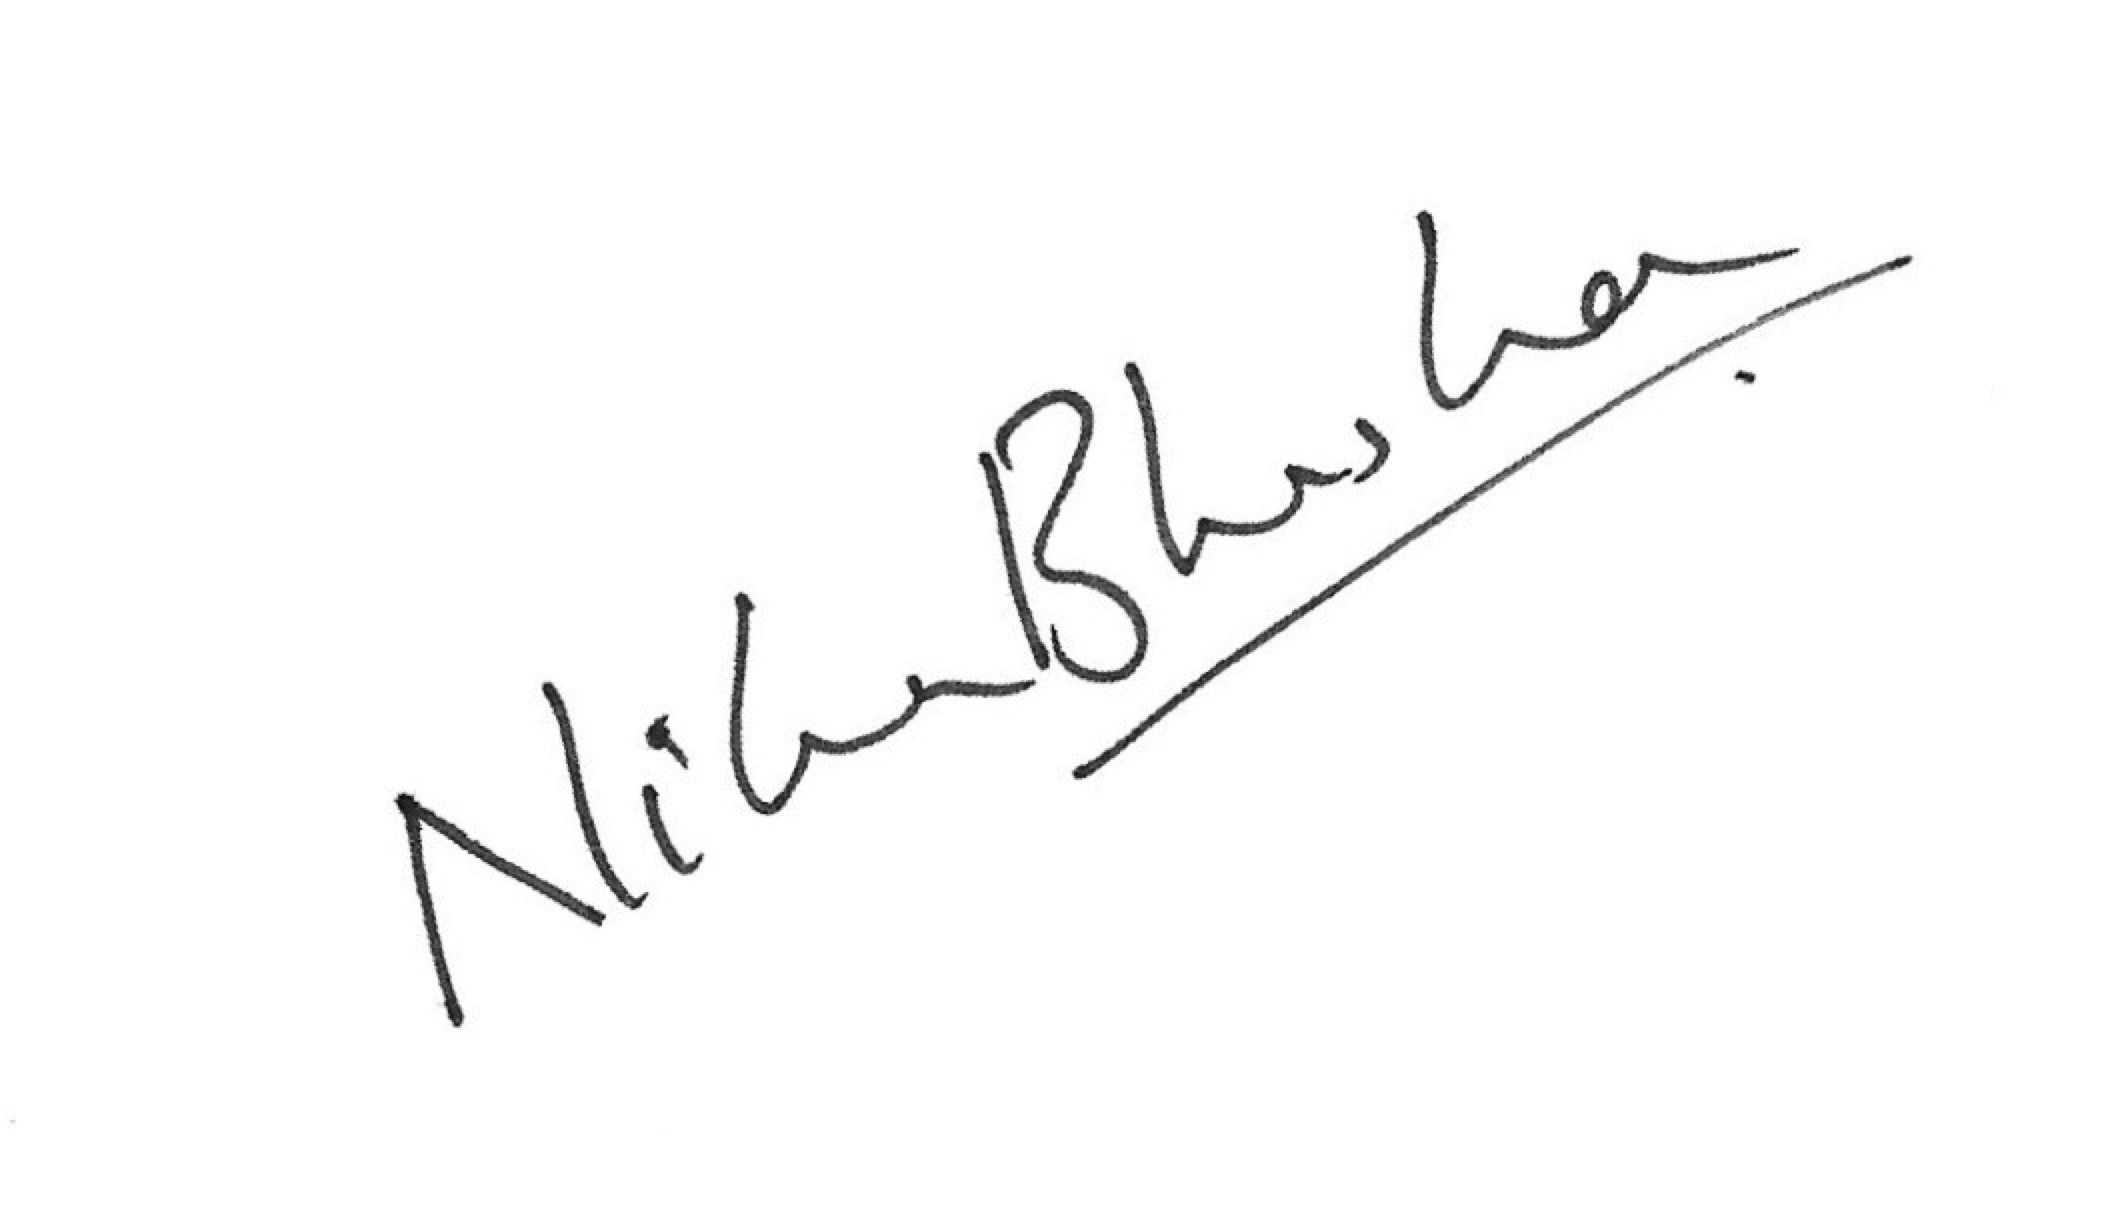
\includegraphics[width=2.5cm,height=1.5cm]{nbhushan_Signature_v2.jpg}\\
Nitin Bhushan \\
%\href{https://nbhushan.github.io}{nbhushan.github.io}
\end{flushleft}


\end{document}